\chapter{Exploratory Data Analysis}
\label{chap:eda}
\chapterguide
  {You should be able to prepare an analysis table and compute grouped summaries.}
  {use distribution, outlier, and relationship summaries to discover structure while separating exploration from confirmation.}

\section{EDA asks what the data are trying to tell you}
\term{Exploratory data analysis (EDA)} is a systematic search for distribution shape, unusual records, group differences, and relationships worth investigating. It is not a licence to report every pattern as a finding.

\begin{utpfig}[EDA lenses]{Move from one variable to pairs and then to conditional or multivariate structure.}{fig:eda-lenses}
\begin{tikzpicture}[x=\linewidth,y=1cm,
  lens/.style={draw=UTPBlue!65,fill=UTPPaleBlue,rounded corners=1.8mm,
    line width=0.7pt,text width=0.235\linewidth,
    minimum width=0.29\linewidth,minimum height=2.20cm,
    inner xsep=4mm,inner ysep=3mm,align=center,
    font=\scriptsize\color{UTPNavy}},
  flow/.style={-{Stealth[length=2mm,width=1.5mm]},
    line width=0.9pt,draw=UTPTeal}]
\node[lens] (u) at (0.17,0)
  {\textcolor{UTPBlue}{\textbf{01  DESCRIBE}}\\[5pt]
   {\footnotesize\textbf{UNIVARIATE}}\\[4pt]
   \textbf{One variable}\\[5pt]
   Shape, centre, and spread};
\node[lens] (b) at (0.50,0)
  {\textcolor{UTPBlue}{\textbf{02  RELATE}}\\[5pt]
   {\footnotesize\textbf{BIVARIATE}}\\[4pt]
   \textbf{Two variables}\\[5pt]
   Differences and relationships};
\node[lens,draw=UTPTeal!80,fill=UTPPaleTeal] (m) at (0.83,0)
  {\textcolor{UTPTeal}{\textbf{03  CONDITION}}\\[5pt]
   {\footnotesize\textbf{MULTIVARIATE}}\\[4pt]
   \textbf{Multiple variables}\\[5pt]
   Patterns within groups\\and joint structure};
\draw[flow] (u.east) -- (b.west);
\draw[flow] (b.east) -- (m.west);
\end{tikzpicture}
\end{utpfig}


\section{Start with shape before choosing a summary}
A mean and standard deviation are informative when the distribution is roughly symmetric and not dominated by extreme values. For skewed or multi-modal distributions, the median, quantiles, and plots often communicate structure more faithfully.

\begin{utpfig}[Three distribution shapes]{Symmetric, skewed, and bimodal distributions can require different summaries and different follow-up questions. Bimodality often suggests hidden groups or multiple data-generating processes.}{fig:eda-shapes}
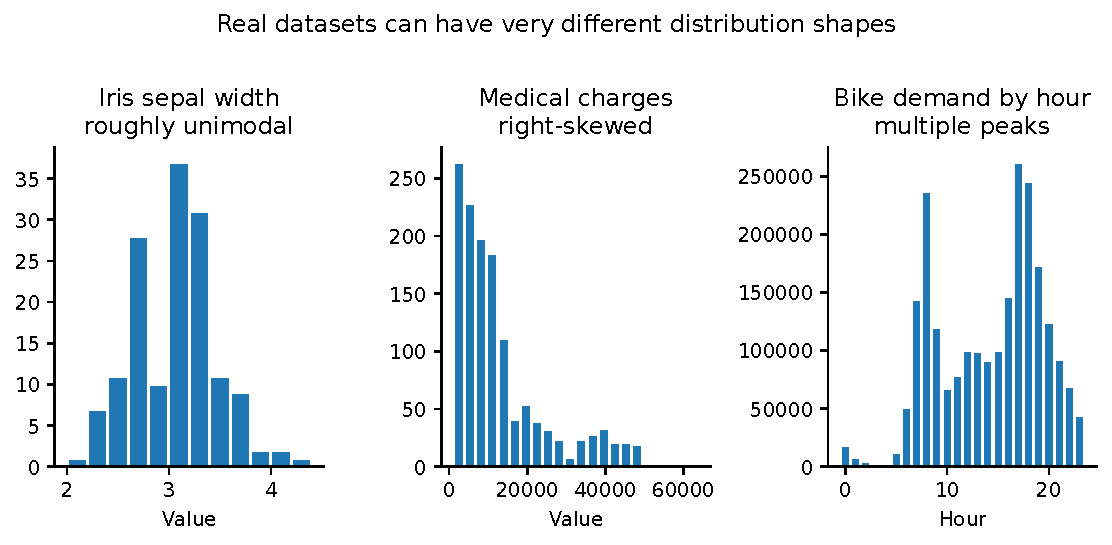
\includegraphics[width=0.90\linewidth]{figures_generated/eda_distribution_shapes.pdf}
\end{utpfig}

A useful first pass records the minimum, lower quartile, median, upper quartile, maximum, mean, standard deviation, missing count, and sample size. The goal is not to report every number, but to notice when the numbers disagree in ways that suggest skew, extreme values, or subgroup structure.

\section{Center without spread is incomplete}
The mean is sensitive to extreme values; the median is more robust. Standard deviation describes typical distance from the mean; the interquartile range (IQR) describes the middle half of the data.

\begin{dstable}
\begin{tabularx}{\linewidth}{@{}D{4.0cm}Y>{\centering\arraybackslash}m{3.0cm}@{}}
\toprule
\rowcolor{DSPaleBlue!92}
\textbf{Statistic} & \textbf{What it describes} & \shortstack{\textbf{Robust to}\\\textbf{extreme values?}} \\
\midrule
Mean & arithmetic center & no \\
Median & middle ordered value & yes \\
Standard deviation & spread around mean & no \\
IQR & spread of middle 50\% & yes \\
Range & minimum to maximum & no \\
\bottomrule
\end{tabularx}
\end{dstable}


\begin{utpfig}[Mean versus median under an outlier]{The mean shifts toward an extreme observation because every value contributes its magnitude. The median depends mainly on order and therefore moves much less.}{fig:eda-mean-median}
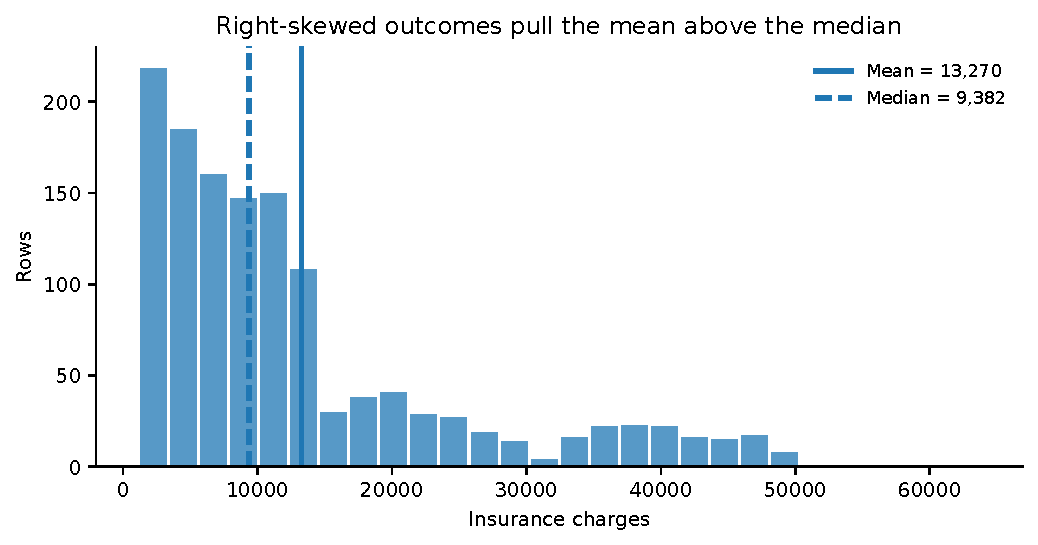
\includegraphics[width=0.84\linewidth]{figures_generated/eda_mean_median_outlier.pdf}
\end{utpfig}

\section{Quantiles describe relative position}
The $p$th quantile is a value below which approximately $p$ proportion of observations fall. Quartiles divide ordered data into four parts; percentiles generalise the same idea. Quantiles are particularly useful for skewed variables because they describe position without assuming symmetry.


\section{Outliers are observations to investigate}
The common 1.5-IQR rule flags values outside
\[
[Q_1 - 1.5\,IQR,\; Q_3 + 1.5\,IQR].
\]
A flag is not a deletion instruction. An extreme observation may be a data error, a rare but valid case, or the most important record in the dataset.

\begin{pitfall}
Deleting outliers because they ``look wrong'' can manufacture a cleaner relationship than the population actually has. Investigate provenance and domain plausibility before removal.
\end{pitfall}


\section{Bivariate EDA depends on variable types}
Different pairs of variable types call for different evidence:
\begin{itemize}
  \item numeric--numeric: scatterplot, correlation, fitted trend, unusual points;
  \item numeric--categorical: side-by-side distributions, group medians/means and spread;
  \item categorical--categorical: contingency tables, conditional proportions, mosaic-style comparisons.
\end{itemize}
The main question is whether the second variable changes the distribution of the first, and whether that change is large enough to matter.


\section{Relationships need visual and numerical evidence}
Correlation summarizes linear association on a scale from -1 to 1. It does not establish causation and can be distorted by nonlinearity, outliers, restricted ranges, or confounding variables.


\begin{utpfig}[Correlation matrix for selected wine measurements]{The matrix summarises pairwise linear association. Strong blocks can reveal redundant features or groups of measurements that move together, but correlation alone does not identify causal relationships.}{fig:eda-corr-heatmap}
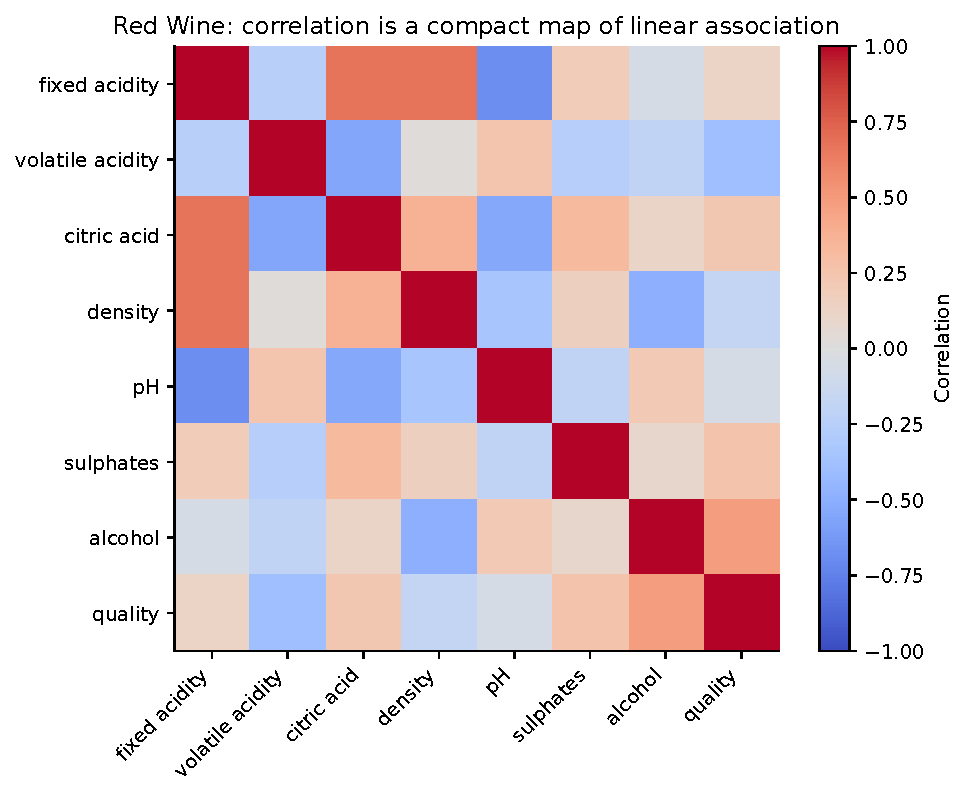
\includegraphics[width=0.74\linewidth]{figures_generated/eda_correlation_heatmap.pdf}
\end{utpfig}

\section{Conditional patterns can reverse an overall pattern}
A relationship in aggregated data can weaken, disappear, or reverse after conditioning on a third variable. This is one reason to examine important relationships within meaningful subgroups. The phenomenon is often associated with \term{Simpson's paradox}: aggregation combines group composition with within-group relationships.

When an overall scatterplot or mean difference seems surprising, ask whether a grouping variable, time period, geography, or data-collection mechanism could be mixing distinct populations.


\begin{workedexample}
If alcohol and colour intensity are correlated in the wine data, plausible explanations include shared chemistry, cultivar differences, or another measured property. A scatterplot coloured or split by cultivar can reveal whether the overall association is partly a group effect.
\end{workedexample}

\section{Exploration versus confirmation}
EDA generates hypotheses. Confirmatory analysis evaluates a question that is sufficiently pre-specified to support formal uncertainty statements. Reusing the same dataset to discover and confirm a pattern tends to overstate certainty.

\begin{keyidea}
Write observations in evidence language: ``The median is higher in group A'' or ``the scatterplot shows a curved relationship.'' Avoid causal language unless the study design supports it.
\end{keyidea}

\section{A repeatable EDA checklist}
\begin{mlsteps}
  \item Verify row count, variable types, missingness, and plausible ranges.
  \item Examine each important numeric distribution and categorical frequency table.
  \item Compare the target or key outcome across relevant groups.
  \item Plot important numeric pairs and inspect correlations cautiously.
  \item Investigate unusual records and record any exclusions.
  \item Summarise three to five evidence-backed observations and open questions.
\end{mlsteps}

\begin{quickcheck}
\begin{enumerate}
  \item When is the median more informative than the mean?
  \item Why is an IQR outlier flag not sufficient reason to delete a row?
  \item Name two ways a correlation can be misleading.
  \item Why should exploratory and confirmatory analysis be distinguished?
\end{enumerate}
\end{quickcheck}

\section{Worked EDA: medical insurance charges}

The Medical Cost Personal dataset is useful because it contains a strongly right-skewed numeric outcome and a subgroup with a large distributional shift. It illustrates why EDA should combine distribution shape, robust summaries, and conditional comparisons.

\begin{utpfig}[Insurance charges: shape before model]{The overall distribution is right-skewed. Splitting by smoking status reveals a much larger shift than an overall histogram alone would communicate.}{fig:eda-medical-costs}
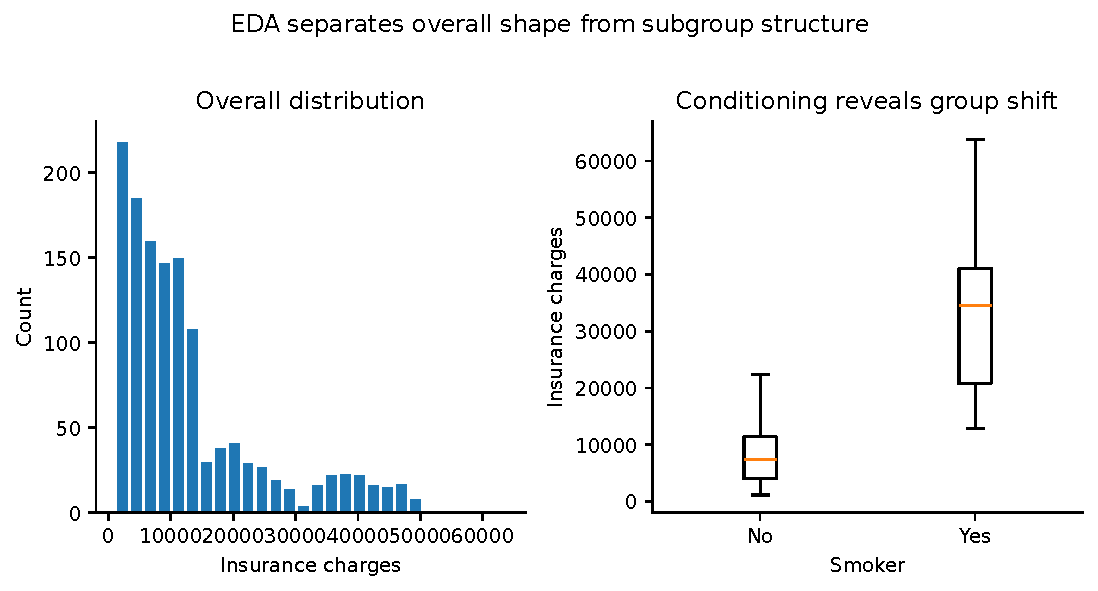
\includegraphics[width=0.90\linewidth]{figures_generated/eda_medical_costs.pdf}
\end{utpfig}

In the bundled file, mean charges are roughly \$8,434 for non-smokers and \$32,050 for smokers; the corresponding medians are about \$7,345 and \$34,456. The difference between mean and median within each group is itself evidence about shape and tail behaviour. Meanwhile the overall BMI--charges correlation is only about 0.20, which does not imply BMI is unimportant: its association can differ by smoking status and age, and nonlinearities or interactions may matter.

\begin{pitfall}
A large group difference discovered during EDA should not be promoted directly to a causal story. Smoking status, age, BMI, and other measured or unmeasured factors are not randomly assigned in this observational dataset.
\end{pitfall}
